% fs-07-Sampling.tex

\documentclass[xcolor=dvipsnames]{beamer}

\usepackage{tikz}
\usepackage{graphicx}
\usepackage{wrapfig}
\usepackage{colortbl}
\usepackage{alltt}
\definecolor{myblue}{rgb}{0.8,0.85,1}

\mode<presentation>
{
  \usetheme{Warsaw}
  \setbeamercovered{transparent}
}
% \usecolortheme[named=OliveGreen]{structure}
\setbeamertemplate{navigation symbols}{} 
\setbeamertemplate{blocks}[rounded][shadow=true] 

\newcounter{expls}
\setcounter{expls}{0}
\newcommand{\beispiel}[1]{\refstepcounter{expls}\textbf{Example \arabic{expls}: #1.}}

\newcounter{exercise}
\setcounter{exercise}{0}
\newcommand{\ubung}[0]{\refstepcounter{exercise}\textbf{Exercise \arabic{exercise}: }}

\makeatletter
\newcommand\binomialCoefficient[2]{%
    % Store values 
    \c@pgf@counta=#1% n
    \c@pgf@countb=#2% k
    %
    % Take advantage of symmetry if k > n - k
    \c@pgf@countc=\c@pgf@counta%
    \advance\c@pgf@countc by-\c@pgf@countb%
    \ifnum\c@pgf@countb>\c@pgf@countc%
        \c@pgf@countb=\c@pgf@countc%
    \fi%
    %
    % Recursively compute the coefficients
    \c@pgf@countc=1% will hold the result
    \c@pgf@countd=0% counter
    \pgfmathloop% c -> c*(n-i)/(i+1) for i=0,...,k-1
        \ifnum\c@pgf@countd<\c@pgf@countb%
        \multiply\c@pgf@countc by\c@pgf@counta%
        \advance\c@pgf@counta by-1%
        \advance\c@pgf@countd by1%
        \divide\c@pgf@countc by\c@pgf@countd%
    \repeatpgfmathloop%
    \the\c@pgf@countc%
}
\makeatother

\newif\ifBCITCourse
\BCITCoursetrue
% \BCITCoursefalse
\newif\ifWhichCourse
\WhichCoursetrue
% \WhichCoursefalse
\ifBCITCourse
\ifWhichCourse
\newcommand{\CourseName}{Statistics for Food Technology}
\newcommand{\CourseNumber}{MATH 2441}
\newcommand{\CourseInst}{BCIT}
\else
\newcommand{\CourseName}{Calculus for Geomatics}
\newcommand{\CourseNumber}{MATH 2511}
\newcommand{\CourseInst}{BCIT}
\fi
\else
\newcommand{\CourseName}{Philosophy and Literature}
\newcommand{\CourseNumber}{PHIL 375}
\newcommand{\CourseInst}{UBC}
\fi

\title{Central Limit Theorem}
\subtitle{{\CourseNumber}, BCIT}

\author{\CourseName}

\date{March 1, 2017}

% \begin{figure}[h]
% 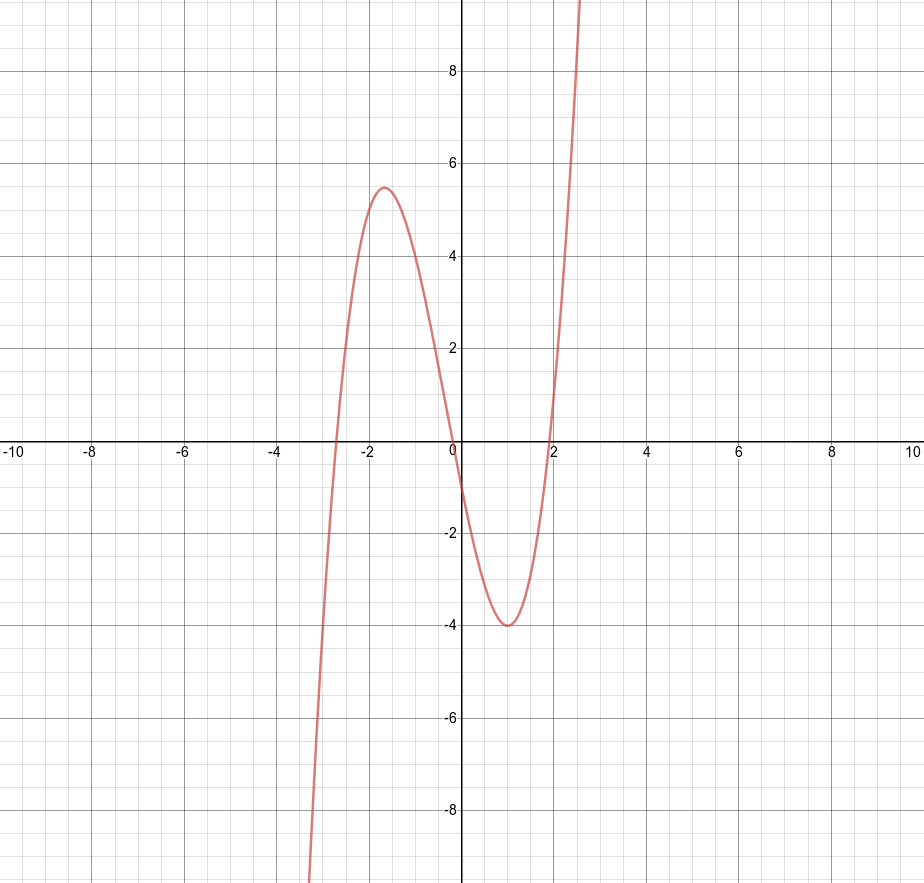
\includegraphics[scale=.3]{./diagrams/extrema1.png}
% \end{figure}

% Command             10pt    11pt    12pt
% \tiny               5       6       6
% \scriptsize         7       8       8
% \footnotesize       8       9       10
% \small              9       10      10.95
% \normalsize         10      10.95   12

\begin{document}

\begin{frame}
  \titlepage
\end{frame}

\begin{frame}
  \frametitle{Sampling Distributions}
So far we have had random variables $X$ which gave us the numerical
results of a random process. Now let's consider a special kind of
random variable $Y$. Let's say you roll a die three times and
\begin{equation}
  \label{eq:quaegieg}
  \left.\begin{array}{rcl}
    X&=&3 \\
    X&=&4 \\
    X&=&1
  \end{array}\right\}Y=\frac{3+4+1}{3}=\frac{8}{3}\notag
\end{equation}
Let's do it again, and we get a different random outcome
\begin{equation}
  \label{eq:iitiloox}
  \left.\begin{array}{rcl}
    X&=&5 \\
    X&=&5 \\
    X&=&2
  \end{array}\right\}Y=\frac{5+5+2}{3}=\frac{12}{3}\notag
\end{equation}
\end{frame}

\begin{frame}
  \frametitle{Sampling Distributions}
The distribution of $Y$ is called a \alert{sampling distribution}. It
can be based on 
\begin{enumerate}
\item the \alert{mean} of a sample
\item the \alert{variance} of a sample
\item the \alert{proportion} of a sample
\end{enumerate}
There is therefore a sampling distribution of the mean, a sampling
distribution of the variance, and a sampling distribution of the
proportion of a population. If I don't want to be specific about which
of the three I am talking about, I will call it the sampling
distribution of a \alert{statistic}.
\end{frame}

\begin{frame}
  \frametitle{Sampling Distributions}
{\ubung} Take a deck of cards and label the cards
$1-52$. Draw five cards with replacement. What are the values for the
sampling distributions (proportion here refers to proportion of
even-numbered cards)?

\medskip

\begin{tabular}{|l|l|l|l|l|l|l|}\hline
  sample \#   & first & second & third & fourth & fifth & sixth \\ \hline
  first card  & 7     & 40     & 18    & 28     & 46    & 40    \\ \hline
  second card & 7     & 17     & 41    & 46     & 33    & 20    \\ \hline
  third card  & 35    & 1      & 41    & 19     & 30    & 48    \\ \hline
  fourth card & 8     & 17     & 16    & 10     & 45    & 18    \\ \hline
  fifth card  & 36    & 18     & 7     & 3      & 22    & 25    \\ \hline
  mean        &       &        &       &        &       &       \\ \hline
  variance    &       &        &       &        &       &       \\ \hline
  proportion  &       &        &       &        &       &       \\ \hline
\end{tabular}
\end{frame}

\begin{frame}
  \frametitle{Sampling Distributions}
{\ubung} Take a deck of cards and label the cards
$1-52$. Draw five cards with replacement. What are the values for the
sampling distributions (proportion here refers to proportion of
even-numbered cards)?

\medskip

\begin{tabular}{|l|l|l|l|l|l|l|}\hline
  sample \#   & first & second & third & fourth & fifth & sixth \\ \hline
  first card  & 7     & 40     & 18    & 28     & 46    & 40    \\ \hline
  second card & 7     & 17     & 41    & 46     & 33    & 20    \\ \hline
  third card  & 35    & 1      & 41    & 19     & 30    & 48    \\ \hline
  fourth card & 8     & 17     & 16    & 10     & 45    & 18    \\ \hline
  fifth card  & 36    & 18     & 7     & 3      & 22    & 25    \\ \hline
  mean        & 18.6  & 18.6   & 24.6  & 21.2   & 35.2  & 30.2  \\ \hline
  variance    & 238.3 & 193.3  & 241.3 & 280.7  & 104.7 & 173.2 \\ \hline
  proportion  & 0.4   & 0.4    & 0.4   & 0.6    & 0.6   & 0.8   \\ \hline
\end{tabular}
\end{frame}

\begin{frame}
  \frametitle{Sampling Distributions}
\begin{tabular}{|l|l|l|l|l|l|l|}\hline
  sample \#   & first & second & third & fourth & fifth & sixth \\ \hline
  first card  & 7     & 40     & 18    & 28     & 46    & 40    \\ \hline
  second card & 7     & 17     & 41    & 46     & 33    & 20    \\ \hline
  third card  & 35    & 1      & 41    & 19     & 30    & 48    \\ \hline
  fourth card & 8     & 17     & 16    & 10     & 45    & 18    \\ \hline
  fifth card  & 36    & 18     & 7     & 3      & 22    & 25    \\ \hline
  mean        & 18.6  & 18.6   & 24.6  & 21.2   & 35.2  & 30.2  \\ \hline
  variance    & 238.3 & 193.3  & 241.3 & 280.7  & 104.7 & 173.2 \\ \hline
  proportion  & 0.4   & 0.4    & 0.4   & 0.6    & 0.6   & 0.8   \\ \hline
\end{tabular}

\medskip

The random variable $X$ has a \alert{uniform distribution} because
the probability of any card to be drawn is $1/52$. The mean of
this probability distribution is $26.5$, the variance is $225.25$,
and the mean proportion of even cards is $0.5$. How good are the
estimates based on the samples? Are they biased?
\end{frame}

\begin{frame}
  \frametitle{Unbiased Estimators}
  \begin{description}
  \item[mean] The \alert{sample mean $\bar{x}$} is an \textbf{unbiased}
    estimator of the \alert{population mean $\mu$} because
  $\mbox{mean}(\bar{x})=\mu$.
\item[variance] The \alert{sample variance $s^{2}$} is an \textbf{unbiased}
    estimator of the \alert{population variance $\sigma^{2}$} because
  $\mbox{mean}(s^{2})=\sigma^{2}$.
\item[proportion] The \alert{sample proportion $\hat{p}$} is an \textbf{unbiased}
    estimator of the \alert{population proportion $p$} because
  $\mbox{mean}(\hat{p})=p$.
\item[st dev] The \alert{sample standard deviation $s$} is a \textbf{biased}
    estimator of the \alert{population standard deviation $\sigma$} because
  $\mbox{mean}(s)\neq\sigma^{2}$.
  \end{description}
  The mean of the sample statistic is taken from all possible ($m$
  choose $n$) samples, where $m$ is the population size and $n$ is the
  sample size.
\end{frame}

\begin{frame}
  \frametitle{Sampling Distributions}
  \beispiel{Sampling in R} First, we roll a die $m=200$ times and plot
  the results. You can see the distribution, which should be
  approximately uniform.
\begin{alltt}
x1<-round((runif(200,0,1)*6)+0.5)\newline
barplot(table(x1))
\end{alltt}
\end{frame}

\begin{frame}
  \frametitle{Sampling Distributions}
  Next, we pick 1000 samples of these 200 die rolls (how many are
  there in total?) and plot their mean. For example, if the sample is
  ``$4,2,5$,'' then the mean is $11/3$. The samples have a sample size
  of $n=3$.
\begin{alltt}
sampling<-function(x) \{\newline
t<-c()\newline
for (i in 1:1000) \{\newline
t<-append(t,mean(sample(x,3)))\newline
\}\newline
return(t)\newline
\}\newline
x2<-sampling(x1)\newline
hist(x2,breaks=seq(1,6,1),col="blue")
\end{alltt}
\end{frame}

\begin{frame}
  \frametitle{Central Limit Theorem}
Given
\begin{enumerate}
\item The original population has mean $\mu$ and standard deviation
  $\sigma$.
\item Simple random samples of the same size $n$ are selected from the population.
\end{enumerate}
Then
\begin{description}
\item[Case 1] Original population is \alert{normally distributed}.
\item[Case 2] Original population is \alert{not normally distributed}.
\end{description}
\end{frame}

\begin{frame}
  \frametitle{Central Limit Theorem}
In \textbf{Case 1}, for \alert{any sample size $n$}, the distribution
of $\bar{x}$ is a \alert{normal distribution} with these parameters.
\begin{enumerate}
\item<1-> The mean of all values of $\bar{x}$ is
\begin{equation}
  \label{eq:wecoutha}
  \mu_{\bar{x}}=\mu
\end{equation}
\item<2-> The standard deviation of all values of $\bar{x}$ is
\begin{equation}
  \label{eq:aunijeeb}
  \sigma_{\bar{x}}=\frac{\sigma}{\sqrt{n}}
\end{equation}
\item<3-> The $z$-score conversion of $\bar{x}$ works according to the
following formula,
\begin{equation}
  \label{eq:aivashah}
  z=\frac{\bar{x}-\mu}{\frac{\sigma}{\sqrt{n}}}
\end{equation}
\end{enumerate}
\end{frame}

\begin{frame}
  \frametitle{Central Limit Theorem}
In \textbf{Case 2}, for \alert{sample sizes $n>30$}, the distribution
of $\bar{x}$ is  \alert{approximately a normal distribution} with these parameters.
\begin{enumerate}
\item The mean of all values of $\bar{x}$ is
\begin{equation}
  \label{eq:chaghiec}
  \mu_{\bar{x}}=\mu
\end{equation}
\item The standard deviation of all values of $\bar{x}$ is
\begin{equation}
  \label{eq:ooloogha}
  \sigma_{\bar{x}}=\frac{\sigma}{\sqrt{n}}
\end{equation}
\item The $z$-score conversion of $\bar{x}$ works according to the
following formula,
\begin{equation}
  \label{eq:yohthoug}
  z=\frac{\bar{x}-\mu}{\frac{\sigma}{\sqrt{n}}}
\end{equation}
\end{enumerate}
\end{frame}

\begin{frame}
  \frametitle{Central Limit Theorem}
In \textbf{Case 2}, for \alert{sample sizes $n\leq{}30$}, the distribution
of $\bar{x}$ cannot be approximated well by a normal distribution and
the methods of this section do not apply.
\end{frame}

\begin{frame}
  \frametitle{Central Limit Theorem Flow Chart}
\begin{figure}[h]
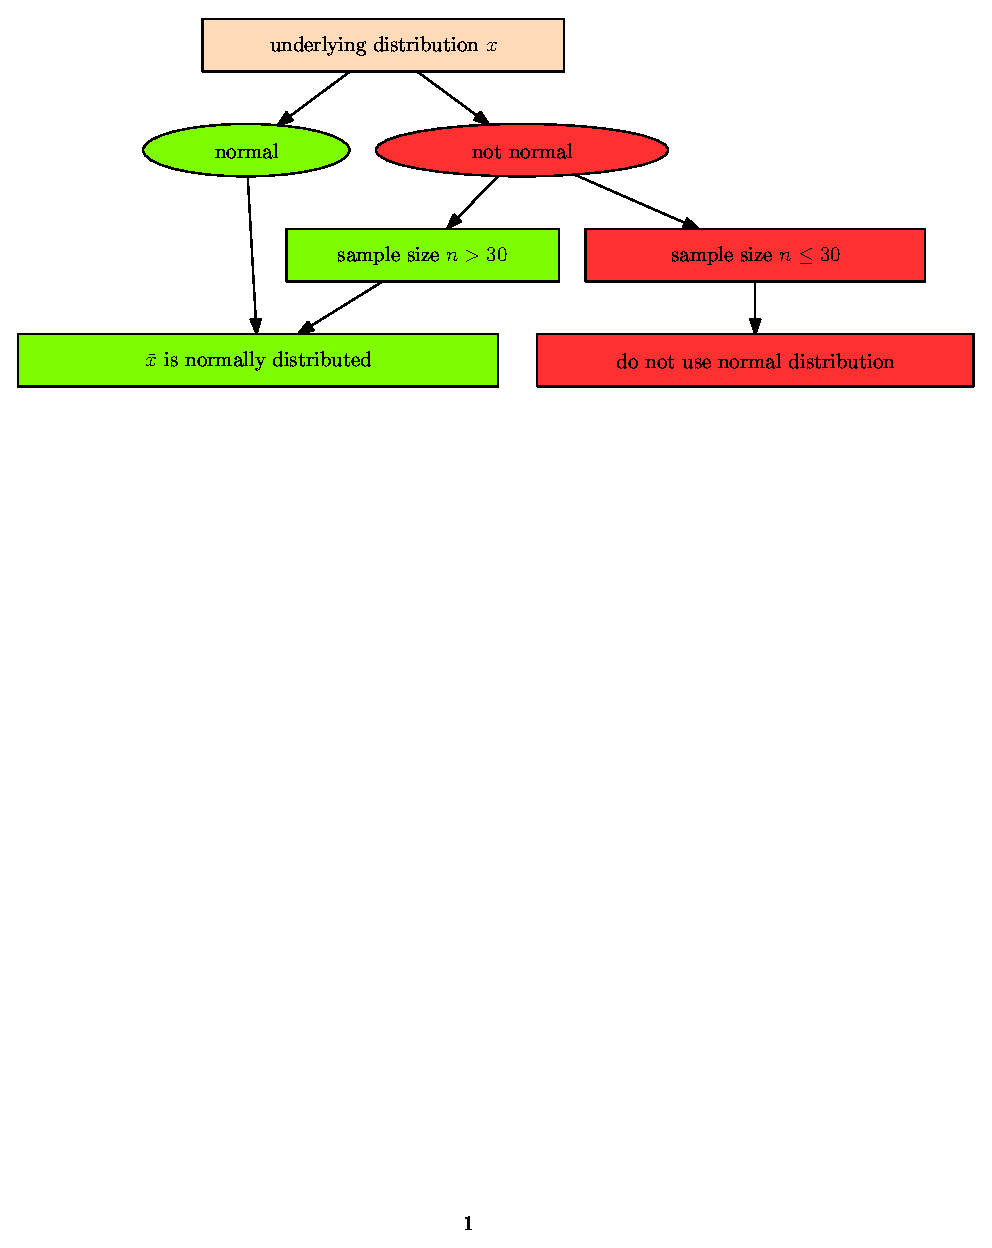
\includegraphics[scale=.7]{./diagrams/CentralLimitTheorem.eps}
\end{figure}
\end{frame}

\begin{frame}
  \frametitle{Correction for a Finite Population}
The Central Limit Theorem assumes that the population is infinite. We
can achieve this by sampling with replacement. In practice, however,
we usually sample without replacement. In this case, all is fine
unless $n>0.05m$, where $m$ is the size of the population. If $n$ is
more than five percent of $m$, we introduce a correction factor so
that
\begin{equation}
  \label{eq:ungeihay}
  \sigma_{\bar{x}}=\frac{\sigma}{\sqrt{n}}\alert{\cdot\sqrt{\frac{m-n}{m-1}}}
\end{equation}

\end{frame}

\begin{frame}
  \frametitle{Central Limit Theorem}
\begin{enumerate}
\item Check Requirements. When working with the mean from a sample,
  verify that the normal distribution can be used by confirming that
  the original population has a normal distribution or $n>30$. 
\item Individual Value or Mean from a Sample? Determine whether you
  are using a normal distribution with a single value $x$ or the mean
  $\bar{x}$ from a sample of $n$ values. 
\end{enumerate}
\end{frame}

\begin{frame}
  \frametitle{Central Limit Theorem}
\begin{description}
\item[Individual Values] When working with an individual value from a
  normally distributed population, use the methods talked about
  earlier with 
  \begin{equation}
    \label{eq:cohseiph}
    z=\frac{x-\mu}{\sigma}
  \end{equation}
\item[Mean from a Sample of Values] When working with a mean for some
  sample of $n$ values, be sure to use the value of $\sigma/\sqrt{n}$
  for the standard deviation of the sample mean, so use
  \begin{equation}
    \label{eq:euruighu}
    z=\frac{\bar{x}-\mu}{\frac{\sigma}{\sqrt{n}}}
  \end{equation}
\end{description}
\end{frame}

\begin{frame}
  \frametitle{Exercises} 
  {\ubung} When designing elevators, an obviously important
  consideration is the weight capacity. An Ohio college student died
  when he tried to escape from a dormitory elevator that was
  overloaded with 24 passengers. The elevator was rated for a capacity
  of 16 passengers with a total weight of 2500 lb. The table below
  shows values of recent adult weight parameters. For the following,
  we assume a worst-case scenario in which all of the passengers are
  males (which could easily happen in a dormitory setting). If an
  elevator is loaded to a capacity of 2500 lb with 16 males, the mean
  weight of a passenger is 156.25 lb.

\medskip

  \begin{tabular}{|l|c|c|}\hline
    & Males & Females \\ \hline
    $\mu$ & 182.9 lb & 165.0 lb \\ \hline
    $\sigma$ & 40.8 lb & 45.6 lb \\ \hline 
    Distribution & normal & normal \\ \hline
  \end{tabular}
\end{frame}

\begin{frame}
  \frametitle{Exercises} 
  {\ubung} When designing elevators, an obviously important
  consideration is the weight capacity. An Ohio college student died
  when he tried to escape from a dormitory elevator that was
  overloaded with 24 passengers. The elevator was rated for a capacity
  of 16 passengers with a total weight of 2500 lb. The table below
  shows values of recent adult weight parameters. For the following,
  we assume a worst-case scenario in which all of the passengers are
  males (which could easily happen in a dormitory setting). If an
  elevator is loaded to a capacity of 2500 lb with 16 males, the mean
  weight of a passenger is 156.25 lb.
  \begin{enumerate}
  \item<1-> Find the probability that one randomly selected adult male
    has a weight greater than 156.25 lb.
  \item<2-> Find the probability that a sample of 16 randomly selected
    adult males has a mean weight greater that 156.25 lb (so that the
    total weight exceeds the maximum capacity of 2500 lb).
  \end{enumerate}
\end{frame}

\begin{frame}
  \frametitle{Exercises} 
\begin{figure}[h]
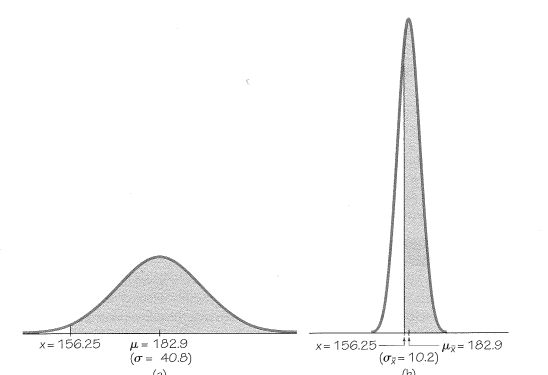
\includegraphics[scale=.75]{./diagrams/triola-281.png}
\end{figure}
\end{frame}

\begin{frame}
  \frametitle{Exercises} 
  {\ubung} You need ro obtain new desks for an incoming class of 25
  kindergarten students who are all 5 years of age. An important
  characteristic of the desks is that the it must accommodate the
  sitting heights of those students. (The sitting height is the height
  of a seated student from the bottom of the feet to the top of the
  knee.) The table below lists the parameters for sitting heights of
  5-year-old children

\medskip

  \begin{tabular}{|l|c|c|}\hline
                 & Boys    & Girls   \\ \hline
    $\mu$        & 61.8 cm & 61.2 cm \\ \hline
    $\sigma$     & 2.9 cm  & 3.1 cm  \\ \hline 
    Distribution & normal  & normal  \\ \hline
  \end{tabular}
\end{frame}

\begin{frame}
  \frametitle{Exercises} 
  {\ubung} You need ro obtain new desks for an incoming class of 25
  kindergarten students who are all 5 years of age. An important
  characteristic of the desks is that the it must accommodate the
  sitting heights of those students. (The sitting height is the height
  of a seated student from the bottom of the feet to the top of the
  knee.) The table below lists the parameters for sitting heights of
  5-year-old children
  \begin{enumerate}
  \item<1-> What sitting height will accommodate 95\% of the boys?
  \item<2-> What sitting height is greater than 95\% of the means of
    sitting heights from random samples of 25 boys?
  \item<3-> Based on the preceding results, what single value should
    be be the minimum sitting height accommodated by the desks? Why
    are the sitting heights of girls not included in the calculations?
  \end{enumerate}
\end{frame}

\begin{frame}
  \frametitle{Exercises} 
\begin{figure}[h]
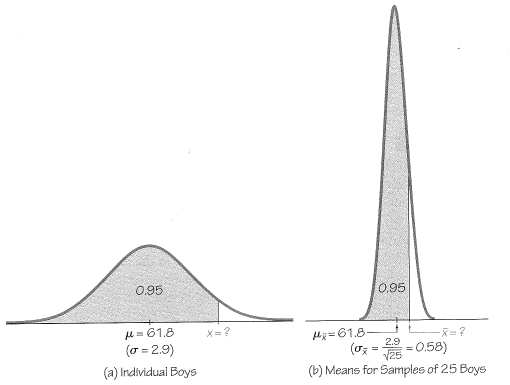
\includegraphics[scale=.75]{./diagrams/triola-284.png}
\end{figure}
\end{frame}

\begin{frame}
  \frametitle{Exercises} 
  {\ubung} Cans of regular Coke are labeled to
  indicate that they contain 12 oz. The corresponding
  sample statistics are $n=36$ and $\bar{x}=12.19$ oz. Assuming that the
  Coke cans are filled so that $\mu=12$ oz (as labeled) and the
  population standard deviation is $\sigma=0.11$ oz (based on the sample
  results), find the probability that a sample of 36 cans will have a
  mean of 12.19 oz or greater. Do these results suggest that the Coke
  cans are filled with an amount greater than 12.00 oz?
\end{frame}

\begin{frame}
  \frametitle{Exercises}
  {\ubung} Women have head circumferences that are normally
  distributed with a mean of 22.65in and a standard deviation of
  0.80in. 
  \begin{enumerate}
  \item<1-> If the hats by Leko company produce women's hats so that
    they fit head circumferences between 21.00in and 25.00in, what
    percentage of women can fit into these hats?
  \item<2-> If the company wants to produce hats to fit all women
    except for those with the smallest 2.5\% and the largest 2.5\%
    head circumferences, what head circumferences should be
    accommodated?
  \item<3-> If 64 women are randomly selected, what is the probability
    that their mean head circumference is between 22.00in and 23.00in?
    If this probability is high, does it suggest that an order for 64
    hats will very likely fit each of 64 randomly selected women? Why
    or why not?
  \end{enumerate}
\end{frame}

\begin{frame}
  \frametitle{Exercises}
  {\ubung} According to the web site www.torchmate.com, ``manhole
  covers must be a minimum of 22in in diameter, but can be as much as
  60in in diameter.'' Assume that a manhole is constructed to have a
  circular opening with a diameter of 22 in. Men have shoulder
  breadths that are normally distributed with a mean of 18.2in and a
  standard deviation of 1.0in (based on data from the National Health
  and Nutrition Examination Survey).
  \begin{enumerate}
  \item<1-> What percentage of men will fit into the manhole?
  \item<2-> Assume that the Connecticut Light and Power company
    employs 36 men who work in manholes. If 36 men are randomly
    selected, what is the probability that their mean shoulder breadth
    is less than 18.5in? Does this result suggest that money can be
    saved by making smaller manholes with a diameter of 18.5in? Why
    or why not?
  \end{enumerate}
\end{frame}

\begin{frame}
  \frametitle{Exercises}
  {\ubung} Passengers died when a water taxi sank in Baltimore's Inner Harbor.
  Men are typically heavier than women and children, so when loading a
  water taxi, assume a worst-case scenario in which all passengers are
  men. Assume that weights of men are normally distributed with a mean
  of 182.9lb and a standard deviation of 40.8lb. The water taxi that
  sank had a stated capacity of 25 passengers, and the boat was rated
  for a load limit of 3500 lb.
\end{frame}

\begin{frame}
  \frametitle{Exercises}
  \begin{enumerate}
  \item<1-> Given that the water taxi that sank was rated for a load
    limit of 3500 lb, what is the mean weight of the passengers if the
    boat is filled to the stated capacity of 25 passengers?
  \item<2-> If the water taxi is filled with 25 randomly selected men,
    what is the probability that their mean weight exceeds the value?
  \item<3-> After the water taxi sank, the weight assumptions were
    revised so that the new capacity became 20 passengers. If the
    water taxi is filled with 20 randomly selected men, what is the
    probability that their mean weight exceeds 175lb, which is the
    maximum mean weight that does not cause the total load to exceed
    3500lb?
  \item<4-> Is the new capacity of 20 passengers safe?
  \end{enumerate}
\end{frame}

\begin{frame}
  \frametitle{Exercises}
  {\ubung} Loading M\&M Packages M\&M plain candies have a mean weight
  of 0.8565g and a standard deviation of 0.0518g. The M\&M candies
  used in a data set came from a package containing 465 candies, and
  the package label stated that the net weight is 396.9g. (If every
  package has 465 candies, the mean weight of the candies must exceed
  $396.9/465=0.8535g$ for the net contents to weigh at least 396.9g.)
  \begin{enumerate}
  \item<1-> If 1 M\&M plain candy is randomly selected, find the
    probability that it weighs more than 0.8535g.
  \item<2-> If 465 M\&M plain candies are randomly selected, find the
    probability that their mean weight is at least 0.8535g.
  \item<3-> Given these results, does it seem that the Mars Company is
    providing M\&M consumers with the amount claimed on the label?
  \end{enumerate}
\end{frame}

\begin{frame}
  \frametitle{Exercises} 
  {\ubung} A ski gondola in Vail, Colorado, carries skiers to the top
  of a mountain. It bears a plaque stating that the maximum capacity
  is 12 people or 2004lb. That capacity will be exceeded if 12 people
  have weights with a mean greater than $2004/12=167$lb. Because men
  tend to weigh more than women, a worst-case scenario involves 12
  passengers who are all men. Assume that weights of men are normally
  distributed with a mean of 182.9 lb and a standard deviation of
  40.8lb.
  \begin{enumerate}
  \item<1-> Find the probability that if an individual man is randomly
    selected, his weight will be greater than 167lb.
  \item<2-> Find the probability that twelve randomly selected men
    will have a mean weight that is greater than 167lb (so that their
    total weight is greater than the gondola maximum capacity of
    2004lb).
  \item<3-> Does the gondola appear to have the correct weight limit?
    Why or why not?
  \end{enumerate}
\end{frame}

\begin{frame}
  \frametitle{Assessing Normality}
  IQ is not a number stenciled onto a person's forehead. Psychologists
  develop tests that are supposed to measure intelligence (and whether
  there is anything to be measured is a matter of controversy). One
  necessary feature of a useful IQ test is that its results are
  normally distributed with a mean of 100 and a standard deviation of
  16 (or 15). You are the manager of a company that creates IQ tests.
  A psychologist introduces a test to you which, applied to a random
  sample of appropriate test subjects, has the following results (next
  slide). The mean is 101.005, the standard deviation is 16.20518.
  Later in the course we will learn that these statistics are
  consistent with the requirement that the test has a mean of 100
  and a standard deviation of 16. The question remains: is the
  data normally distributed?
\end{frame}

\begin{frame}
  \frametitle{Assessing Normality}
\begin{footnotesize}
\begin{tabular}{|rrrrrrrrrr|}\hline
104 & 127 & 91  & 91  & 87  & 113 & 112 & 100 & 97  & 87  \\
78  & 99  & 87  & 88  & 103 & 95  & 102 & 104 & 114 & 87  \\
63  & 93  & 106 & 110 & 82  & 97  & 102 & 100 & 107 & 91  \\
105 & 109 & 103 & 115 & 95  & 95  & 128 & 92  & 120 & 107 \\
121 & 81  & 101 & 102 & 105 & 119 & 82  & 105 & 73  & 115 \\
116 & 95  & 85  & 119 & 113 & 108 & 160 & 128 & 101 & 69  \\
87  & 104 & 78  & 85  & 93  & 95  & 128 & 85  & 83  & 82  \\
124 & 67  & 106 & 126 & 106 & 103 & 105 & 98  & 76  & 128 \\
104 & 122 & 105 & 90  & 110 & 86  & 82  & 87  & 100 & 108 \\
83  & 118 & 102 & 109 & 80  & 78  & 112 & 89  & 113 & 92  \\
107 & 79  & 111 & 111 & 102 & 84  & 101 & 82  & 93  & 87  \\
108 & 113 & 131 & 108 & 87  & 89  & 83  & 92  & 117 & 95  \\
85  & 104 & 114 & 113 & 78  & 120 & 102 & 114 & 74  & 97  \\
103 & 88  & 90  & 124 & 92  & 120 & 81  & 91  & 139 & 115 \\
142 & 99  & 119 & 87  & 109 & 73  & 94  & 95  & 91  & 101 \\
101 & 122 & 89  & 107 & 118 & 108 & 97  & 109 & 123 & 125 \\
107 & 89  & 117 & 105 & 122 & 92  & 91  & 44  & 106 & 74  \\
133 & 125 & 95  & 111 & 128 & 74  & 97  & 112 & 79  & 107 \\
127 & 104 & 98  & 109 & 99  & 101 & 104 & 121 & 99  & 119 \\
94  & 119 & 84  & 87  & 94  & 92  & 93  & 86  & 104 & 113 \\ \hline
\end{tabular}
\end{footnotesize}
\end{frame}

\begin{frame}
  \frametitle{Assessing Normality}
To assess normality, we follow a three-step procedure.
\begin{description}
\item[Histogram] Construct a histogram. If the histogram departs
  dramatically from a bell shape, conclude that the data does not
  have a normal distribution.
\item[Outliers] Use a boxplot to identify outliers. If there is
  more than one outlier present, conclude that the data does not
  have a normal distribution.
\item[NQP] If the data passes the first two
  tests, use technology to generate a \alert{normal quantile
    plot}. The population is probably not normally distributed if
  either one of the following two conditions apply:
  \begin{enumerate}
  \item The points do not lie reasonably close to a straight line.
  \item The points show some systematic pattern that is not a
    straight-line pattern.
  \end{enumerate}
\end{description}
\end{frame}

\begin{frame}
  \frametitle{Histogram}
\begin{figure}[h]
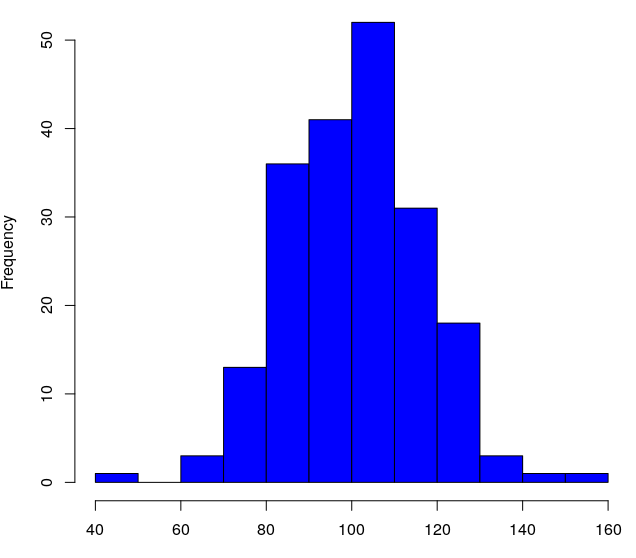
\includegraphics[scale=.4]{./diagrams/an-hist.png}
\end{figure}
\end{frame}

\begin{frame}
  \frametitle{Boxplot}
\begin{figure}[h]
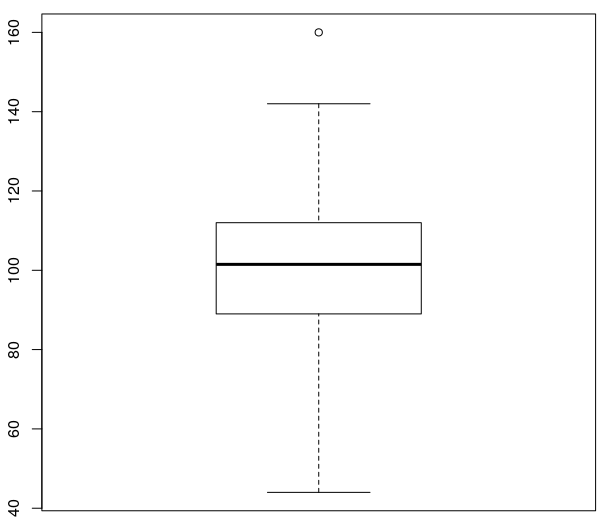
\includegraphics[scale=.4]{./diagrams/an-box.png}
\end{figure}
\end{frame}

\begin{frame}
  \frametitle{Normal Quantile Plot}
\begin{figure}[h]
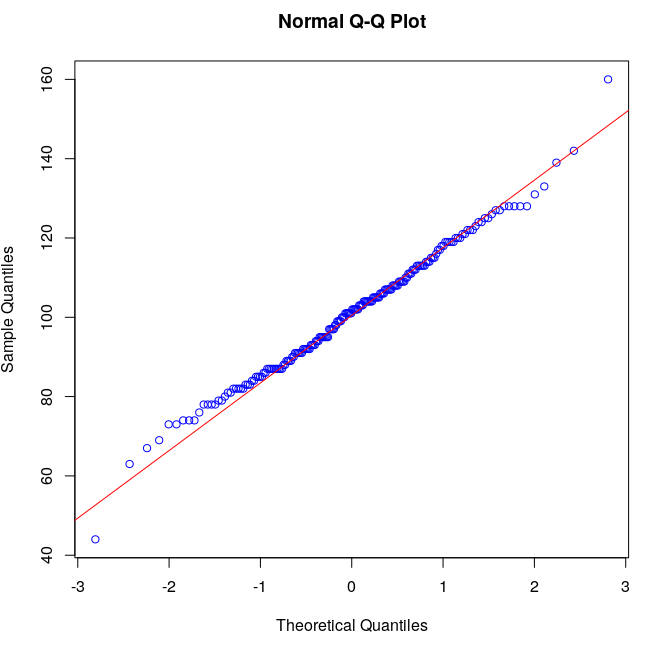
\includegraphics[scale=.35]{./diagrams/an-nqp.png}
\end{figure}
\end{frame}

\begin{frame}
  \frametitle{R Code}
  The following R Statistics code will generate normal data and
  the graphs associated with each of the three steps.
\begin{alltt}
x<-round(rnorm(200,100,16),0)\newline
hist(x,col="blue")\newline
boxplot(x,range=2)\newline
qqnorm(x,col="blue")\newline
qqline(x,col="red")
\end{alltt}
\end{frame}

\begin{frame}
  \frametitle{Non-Normal Distributions}
  Try the following R Statistics code for some non-normal
  distributions.
\begin{alltt}
y<-round(runif(200,50,150),0)\newline
w<-rnorm(200,0,20)\newline
z<-100-(((abs(w)/w)*50)-w)\newline
v<-rnorm(200,500,40)\newline
v<-append(v,rnorm(200,300,40))
\end{alltt}
\texttt{y} is a uniform distribution, \texttt{z} is a U-shaped
distribution (\texttt{w} helps to generate \texttt{z}), and \texttt{v}
is a two-peaked distribution.
\end{frame}

\begin{frame}
  \frametitle{Histogram of Uniform Distribution}
\begin{figure}[h]
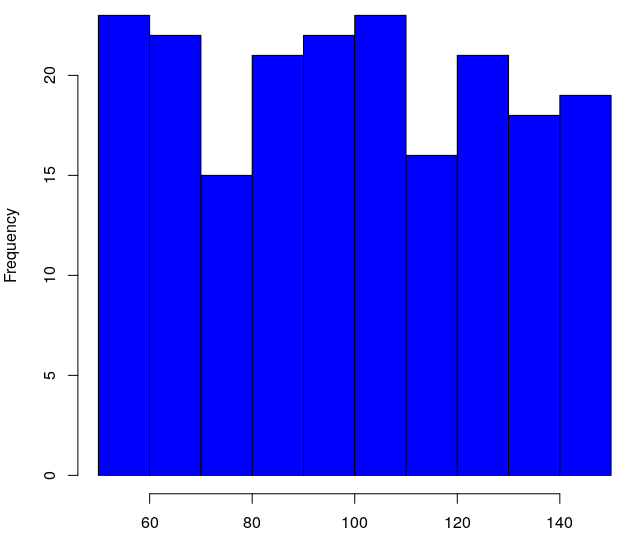
\includegraphics[scale=.4]{./diagrams/an-histunif.png}
\end{figure}
\end{frame}

\begin{frame}
  \frametitle{Normal Quantile Plot of Uniform Distribution}
\begin{figure}[h]
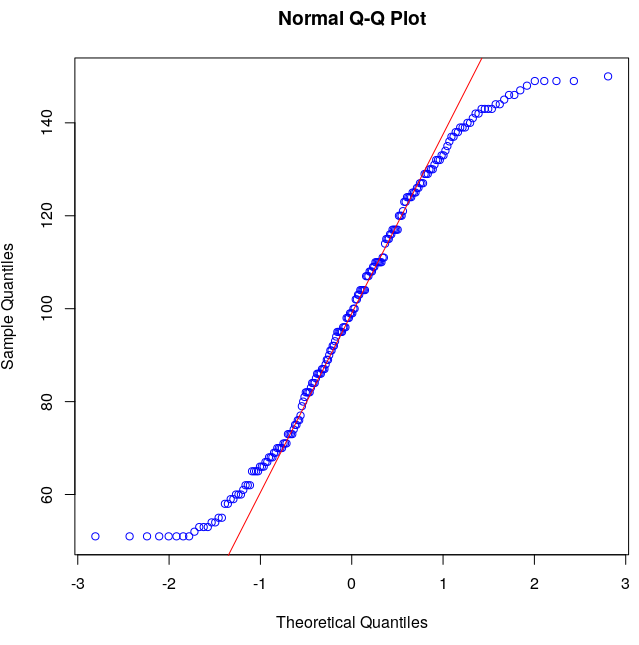
\includegraphics[scale=.35]{./diagrams/an-unif.png}
\end{figure}
\end{frame}

\begin{frame}
  \frametitle{Histogram of U-Shaped Distribution}
\begin{figure}[h]
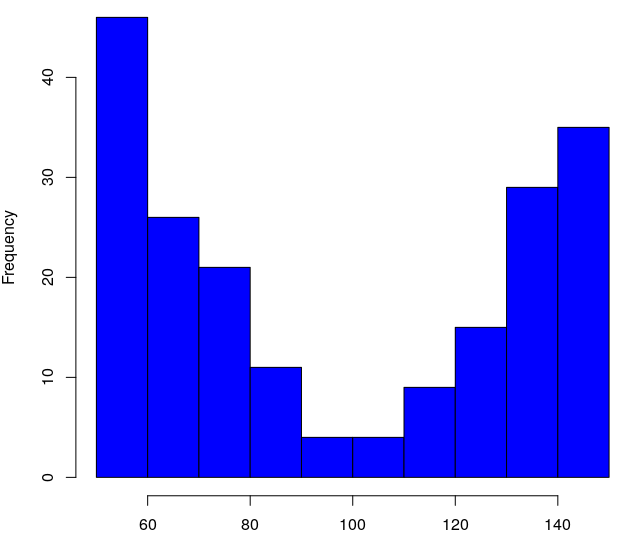
\includegraphics[scale=.4]{./diagrams/an-uhist.png}
\end{figure}
\end{frame}

\begin{frame}
  \frametitle{Normal Quantile Plot of U-Shaped Distribution}
\begin{figure}[h]
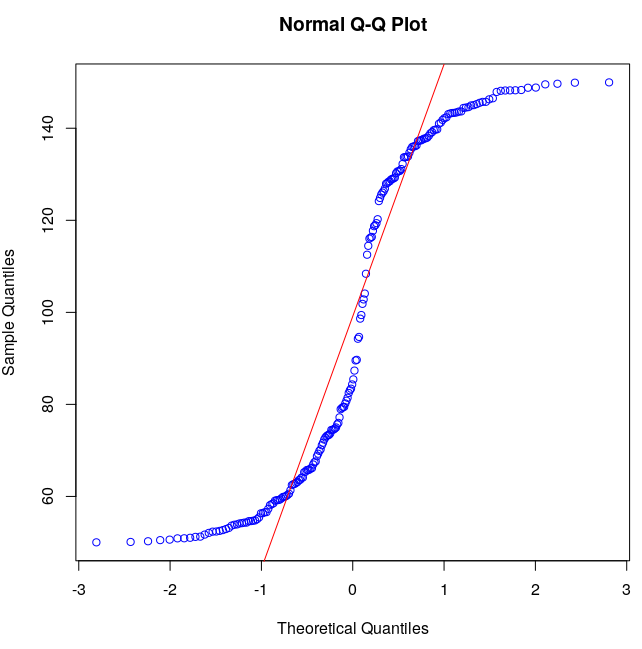
\includegraphics[scale=.35]{./diagrams/an-unqp.png}
\end{figure}
\end{frame}

\begin{frame}
  \frametitle{Histogram of Two-Peaked Distribution}
\begin{figure}[h]
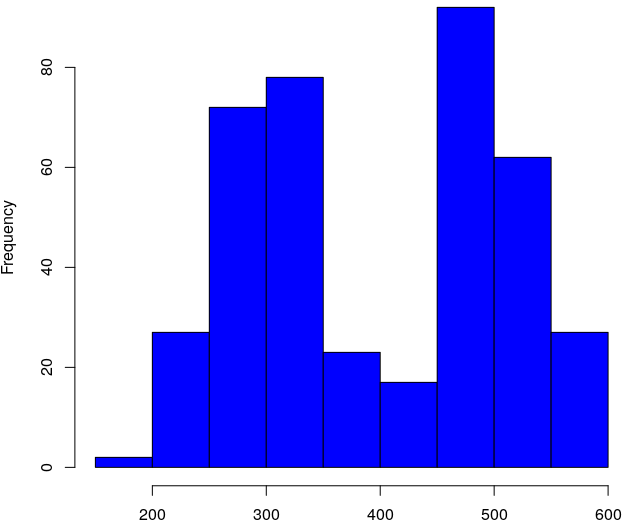
\includegraphics[scale=.4]{./diagrams/an-2phist.png}
\end{figure}
\end{frame}

\begin{frame}
  \frametitle{Normal Quantile Plot of Two-Peaked Distribution}
\begin{figure}[h]
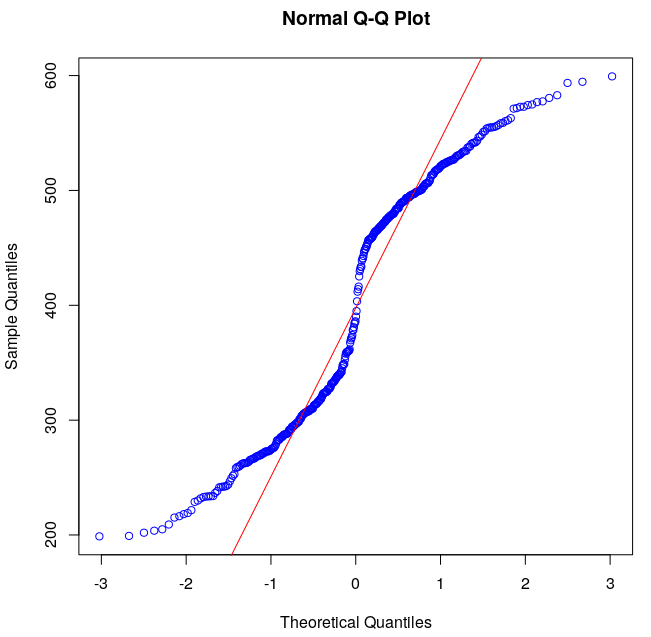
\includegraphics[scale=.35]{./diagrams/an-2pnqp.png}
\end{figure}
\end{frame}

\begin{frame}
  \frametitle{Guess the Number of Jelly Beans}
\begin{figure}[h]
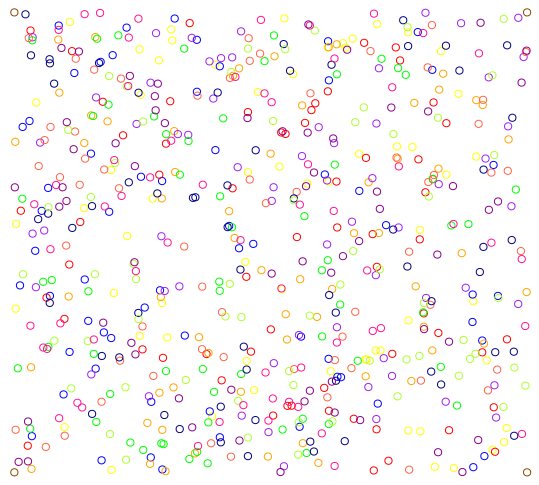
\includegraphics[scale=.4]{./diagrams/an-jb.png}
\end{figure}
% 675
\end{frame}

\begin{frame}
  \frametitle{Exercises}
  {\ubung} Follow the three-step procedure to find out if the
  following data sets are normally distributed. You can find the
  data on D2L.
  \begin{enumerate}
  \item Ages of Oscar-Winning Actresses \texttt{OSCRF.TXT}
  \item Body Temperatures \texttt{BTEMP.TXT}
  \item White Blood Cell Counts for Males \texttt{MWHT.TXT}
  \item Flight Departure Delays \texttt{DPDLY.TXT}
  \end{enumerate}
\end{frame}

\begin{frame}
  \frametitle{End of Lesson}
Next Lesson: One Population
\end{frame}

\end{document}
